\chapter{Извлечение признаков}

Лектор: Алексей Сергеевич Забашта

\section{Метод главных компонент}

\begin{definition}
    \textbf{Метод главных компонент} (\textit{Principal Components Analysis}, \textit{PCA}) — один из основных способов уменьшить размерность данных, потеряв наименьшее количество информации.
\end{definition}

В одномерном случае дано множество точек в $\R^n$ и требуется описать эти данные при помощи одной переменной. Это задача регрессии без учителя. Идея решения ---  проецировать на прямую, такую, что:
\begin{enumerate}
    \item расстояние от точек до нее минимально;
    \item дисперсия проекций максимальна.
\end{enumerate}
\begin{remark}
    Эти условия эквивалентны.
\end{remark}

\begin{figure}
    \centering
    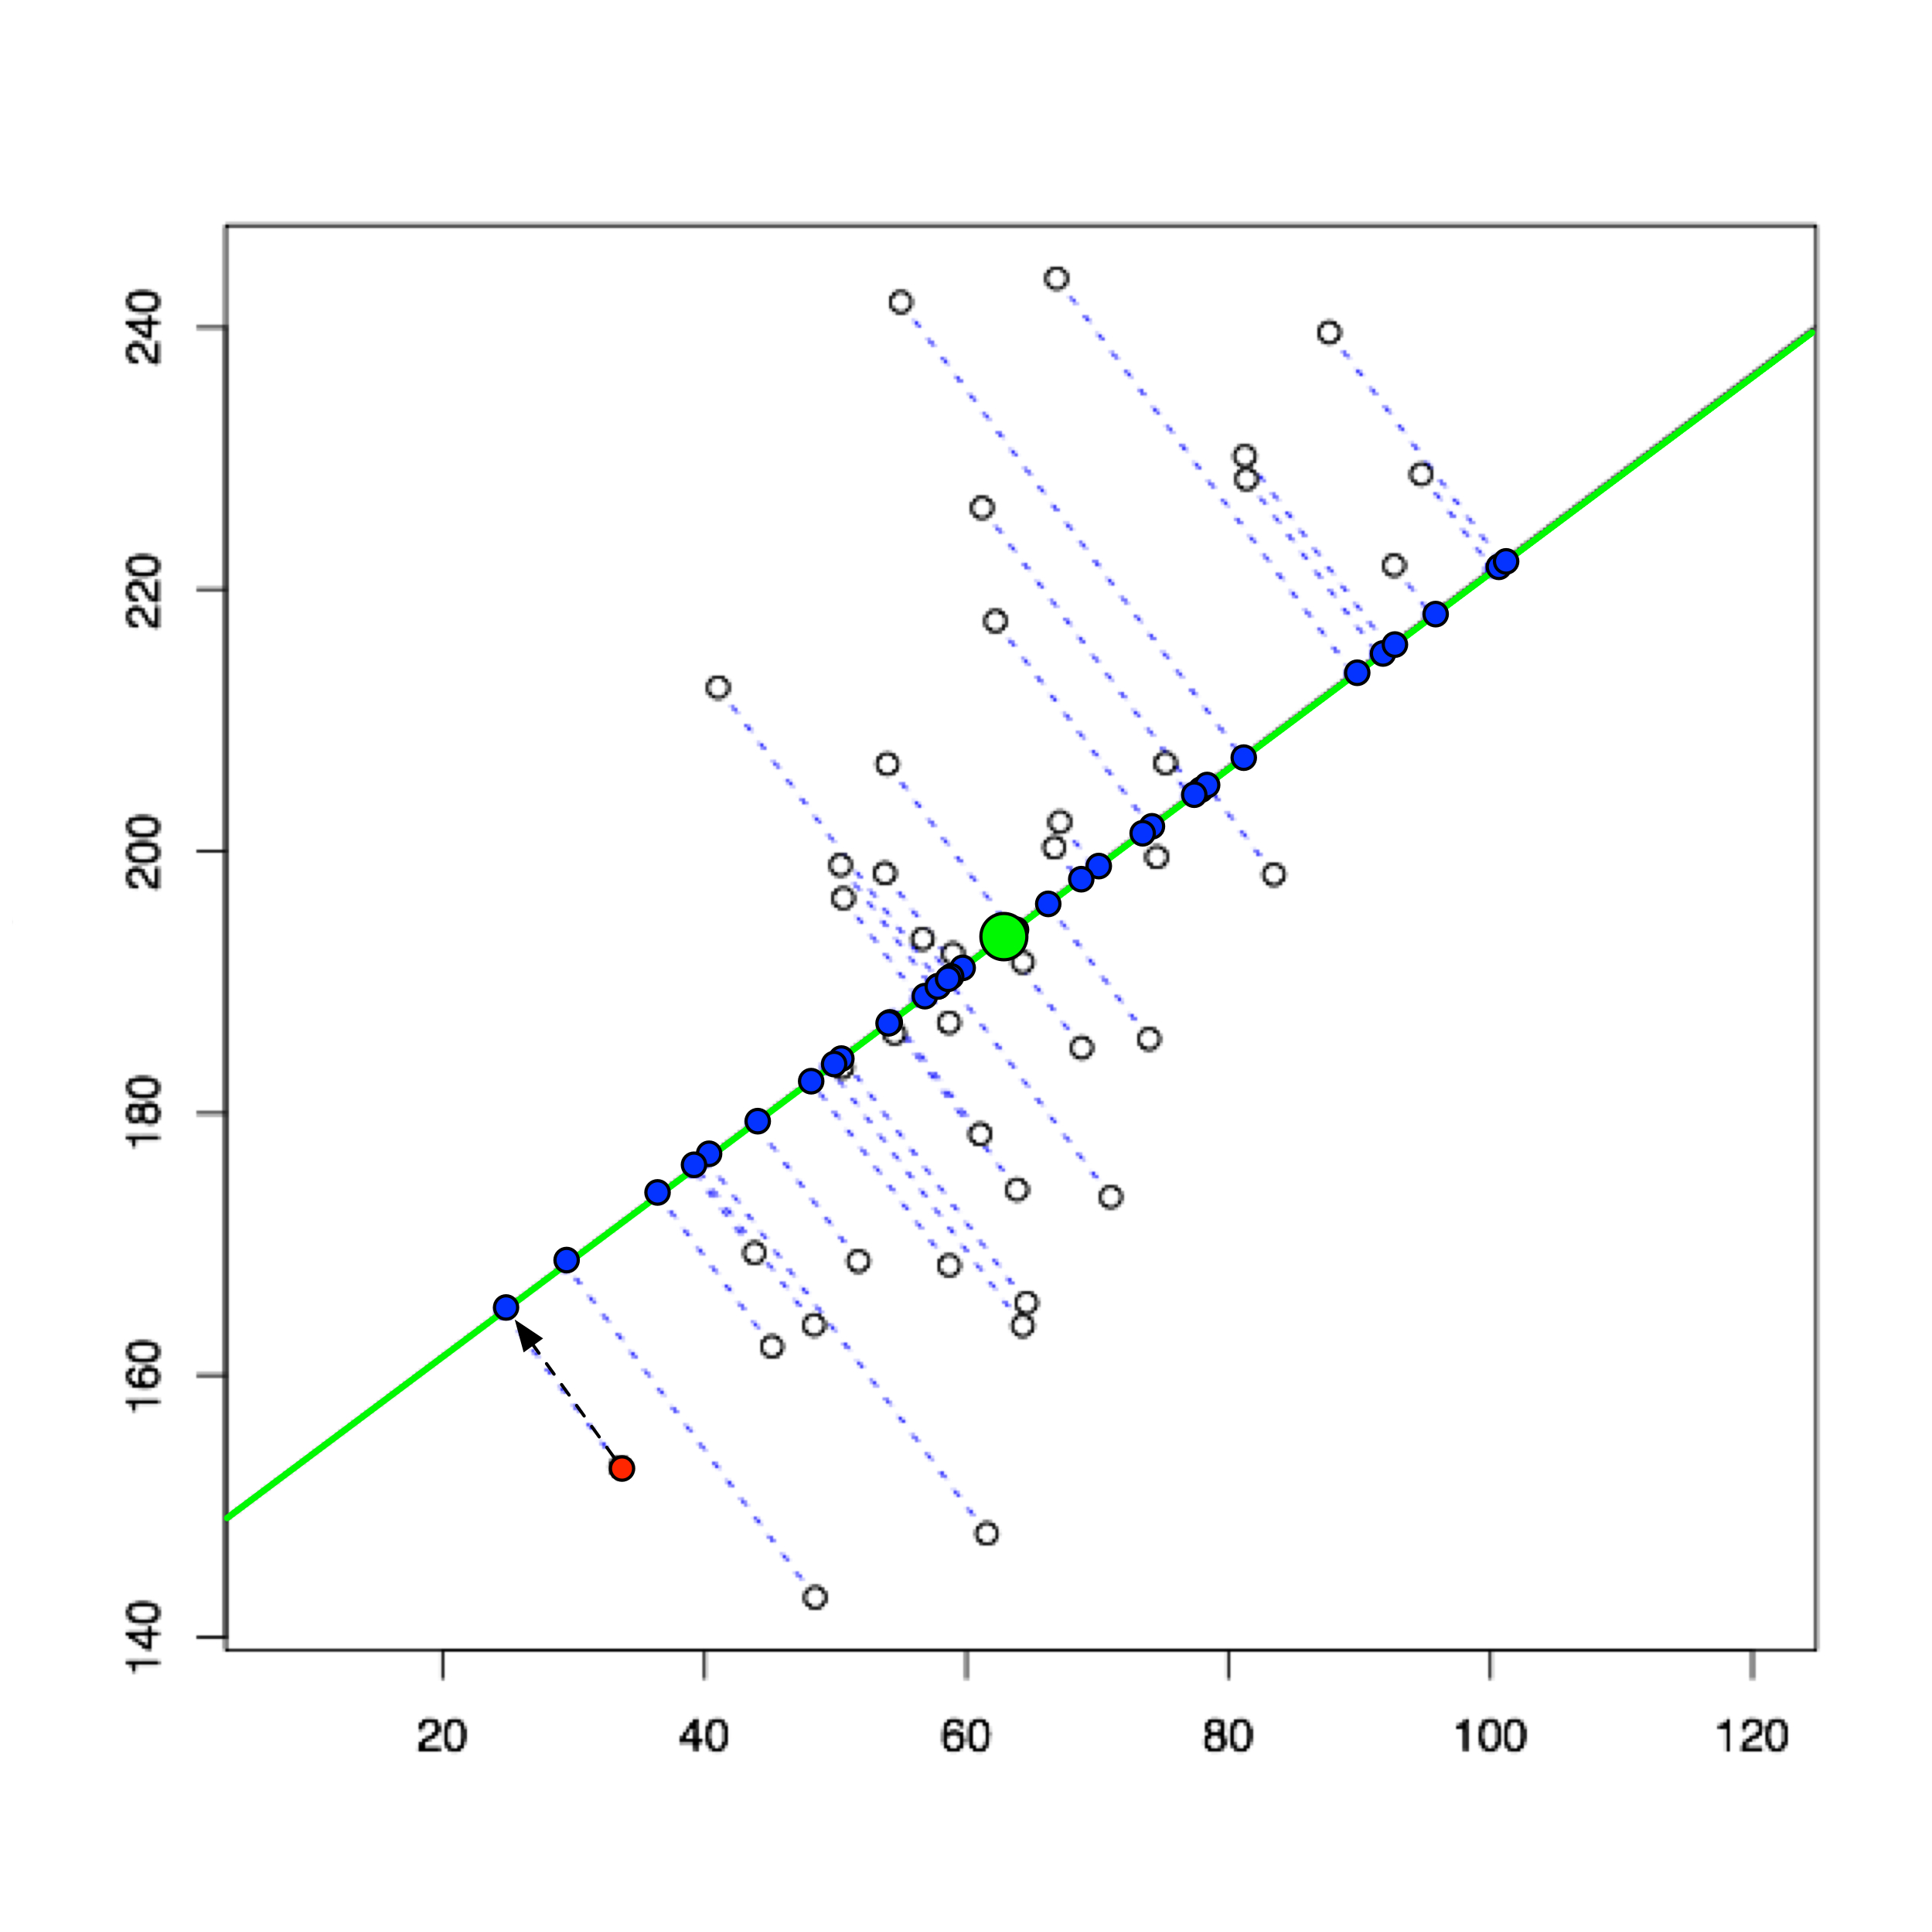
\includegraphics[width=0.6\textwidth]{images/pca-example.jpg}
    \caption{Иллюстрация одномерного случая}
\end{figure}

В общем случае стоит задача приблизить данные линейным многообразием меньшего размера, с требованиями к решению:
\begin{itemize}
    \item Минимизация расстояния;
    \item Максимизация дисперсии проекций;
    \item Максимизация расстояний между проекциями;
    \item Корреляция между осями проекций равна нулю.
\end{itemize}

\begin{remark}
    Существует много вариантов того, как можно описать требования к решению.
\end{remark}

Формальная постановка задачи такова. Имеется $n$ числовых признаков $f_j(x)$, $j=1,...,n$. Объекты обучающей выборки отождествляются с их признаковыми описаниями: $x\equiv(f_1(x_i),...,f_n(x_i))$, $i=1,...,l$. Рассмотрим матрицу $F$, строки которой соответствуют признаковым описаниям обучающих объектов:
\[
    F_{l\times n}=
    \begin{pmatrix}
        f_1(x_1) & ... & f_n(x_1) \\
          ...    & ... &   ...    \\
        f_1(x_l) & ... & f_n(x_l)
    \end{pmatrix}=
    \begin{pmatrix}
        x_1 \\
        ... \\
        x_l
    \end{pmatrix}.
\]
Обозначим $z_i=(g_1(x_i),...,g_m(x_i))$ признаковые описания тех же объектов в новом пространстве $Z=\R^m$ меньшей размерности $m<n$:
\[
    G_{l\times m}=
    \begin{pmatrix}
        g_1(x_1) & ... & g_m(x_1) \\
          ...    & ... &   ...    \\
        g_1(x_l) & ... & g_m(x_l)
    \end{pmatrix}=
    \begin{pmatrix}
        z_1 \\
        ... \\
        z_l
    \end{pmatrix}.
\]

Потребуем, чтобы исходные признаковые описания можно было восстановить по новым описаниям с помощью некоторого линейного преобразования, определяемого матрицей $U=(u_{js})_{n\times m}$:
\[
    \widehat{f}_j(x)=\sum_{s=1}^mg_s(x)u_{js},\quad j=1,...,n,\quad x\in X,
\]
или в векторной записи $\widehat{x}=zU^T$.
\begin{remark}
    Восстановленное описание $\widehat{x}$ не обязано в точности совпадать с исходным описанием $x$, но их отличие на объектах обучающей выборки должно быть как можно меньше при выбранной размерности $m$.
\end{remark}

Будем искать одновременно и матрицу новых признаковых описаний $G$, и матрицу линейного преобразования $U$, при которых суммарная невязка $\Delta^2(G,U)$ восстановленных описаний минимальна:
\[
    \Delta^2(G,U)=\sum_{i=1}^l||\widehat{x}_i-x_i||^2=\sum_{i=1}^l||z_iU^T-x_i||^2=||GU^T-F||^2\to\min_{G,U},
\]
где все нормы евклидовы.
Будем предполагать, что матрицы $G$ и $U$ не вырождены: $\mathrm{rank}G=\mathrm{rank}U=m$. Иначе существовало бы представление $\bar{G}\bar{U}^T=GU^T$ с числом столбцов в матрице $\bar{G}$, меньшим $m$. Поэтому интересны лишь случаи, когда $m\leq\mathrm{rank}F$.

\begin{theorem}
    Если $m\leq\rank F$, то минимум $\Delta^2(G,U)$ достигается, когда столбцы матрицы $U$ есть собственные векторы $F^TF$, соответствующие $m$ максимальным собственным значениям. При этом $G=FU$, матрицы $U$ и $G$ ортогональны.
\end{theorem}

\begin{remark}
    Доказательство можно найти на вики-конспектах.
\end{remark}

\begin{remark}
    Подразумевается, что данные были нормализованы, поэтому $F^TF$ является матрицей корреляции.
\end{remark}

\textit{Следствия}:
\begin{enumerate}
    \item $U^TU=E_m$ --- единичная матрица;
    \item $G^TG=\Lambda=\mathrm{diag}(\lambda_1,...,\lambda_m)$;
    \item $U\Lambda=F^TFU$, $G\Lambda=F^TFG$;
    \item $||GU^T-G||^2=||F||^2 - \mathrm{tr}\Lambda=\sum_{i=m+1}^n\lambda_i$
\end{enumerate}

Таким образом, если отсортировать собственные значения $F^TF$ по убыванию: $\lambda_{(1)}\geq...\geq\lambda_{(n)}$, то
\[
    E(k)=\dfrac{||GU^T-F||^2}{||F||^2}=\dfrac{\lambda_{(k+1)}+...+\lambda_{(n)}}{\lambda_{(1)}+...+\lambda_{(n)}}
\]
характеризует долю информации, теряемую при проекции, поэтому значение $k$ можно выбирать по $E(k)$.

\begin{remark}
    Главные компоненты можно искать итеративно. Сначала необходимо найти прямую $c_1$ расстояние до которой минимально. Затем на каждой итерации искать прямую $c_i$, ортогональную ${c_j}_{j=1}^{i-1}$, расстояние до которой минимально.
\end{remark}

Таким образом, PCA --- это линейное преобразование со всеми достоинствами и недостатками, оно работает быстро и широко распространено для сжатия данных и визуализации. Улучшить его можно, используя нелинейные методы (главные кривые и главные многообразия).\newline
Вариации и родственники PCA:
\begin{itemize}
    \item Анализ независимых компонент (ICA);
    \item EM PCA;
    \item Ядерный PCA;
    \item Канонический корреляционный анализ (CCA).
\end{itemize}

\section{Автокодировщики}

\begin{definition}
    \textbf{Автокодировщик} (\textit{autoencoder}) --- это глубокая нейронная сеть, способная строить низкоразмерные представления данных за счет нелинейной трансформации. Основная идея заключается в том чтобы заставить сеть предсказывать (восстанавливать) то, что подается ей на вход, ограничив возможность обучиться тривиальному преобразованию.
\end{definition}

Существует два варианта ограничения преобразования:
\begin{enumerate}
    \item Структурный: между входными и выходными слоями должен быть слой меньшей размерности, так называемое \textbf{бутылочное горлышко} (\textit{bootleneck}). Это \textbf{недополненный (undercomplete) автокодировщик}.
    \item Регуляризационный: добавим регуляризационную константу к выходам этого слоя, уменьшающим его размерность. Это \textbf{разреженный (sparce) автокодировщик}.
\end{enumerate}

\begin{figure}[h]
    \centering
    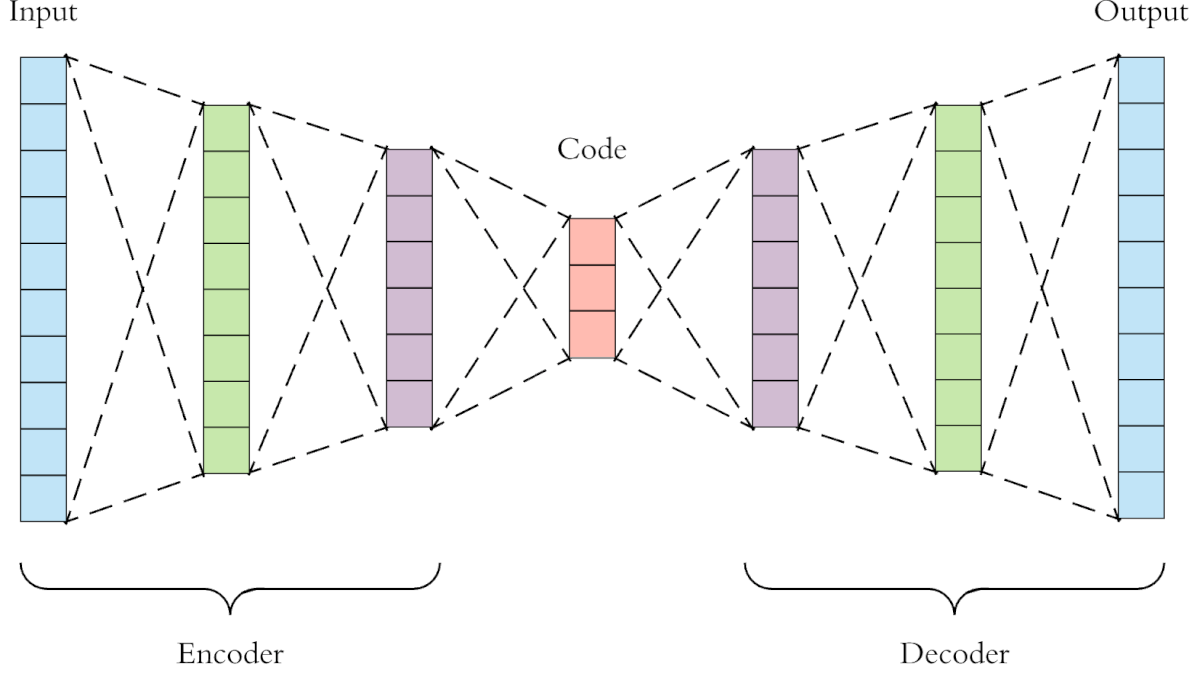
\includegraphics[width=\textwidth]{images/autoencoder.png}
    \caption{Архитектура автоэнкодера}
\end{figure}

\begin{definition}
    \textbf{Кодировщик} (\textit{encoder}) --- часть сети от входного слоя до бутылочного горлышка.
\end{definition}

\begin{definition}
    \textbf{Декодировщик} (\textit{decoder}) --- часть сети от бутылочного горлышка до выходного слоя.
\end{definition}

Пусть $c$ --- кодировщик, $d$ --- декодировщик, $L$ --- некая регуляризация, $\tau$ --- коэффициент регуляризации. Минимизировать будем не $||d(c(x))-x||$, а
\[
    ||d(c(x))-x||+\tau\cdot L(c(x))
\]

\begin{remark}
    Стандартно можно взять $L_1$ норму.
\end{remark}

Вариации автокодировщика:
\begin{itemize}
    \item Шумоподавляющий (denoising) автокодировщик;
    \item Сжимающий (contractive) автокодировщик;
    \item Вариационный (variational) автокодировщик (основан на совсем других принципах).
\end{itemize}

\section{t-SNE}

\begin{definition}
    \textbf{Стохастическое вложение соседей с t-распределением} (\textit{t-distributed stochastic neighbor embedding}, \textit{t-SNE}) --- нелинейный алгоритм улучшения размерности, который используется для визуализации и пытается сохранять метрические отношения между объектами:
    \begin{enumerate}
        \item Определяется вероятность для точки "выбрать ближайшим соседом" другую точку в пространстве;
        \item Строятся такие распределения для высокоразмерных и низкоразмерных представлений.
        \item Минимизируется расстояние Кульбака-Лейблера между этими двумя распределениями.
    \end{enumerate}
\end{definition}

\begin{definition}
    \textbf{Расстояние (дивергенция) Кульбака-Лейблера} (\textit{KL divergence}) --- расстояние между двумя распределениями $P$ и $Q$:
    \[
        D_{KL}(P||Q)=\int_{-\infty}^{+\infty}p(x)\log\dfrac{p(x)}{q(x)}d(x),
    \]
    где $p$ распределено согласно $P$, а $q$ --- согласно $Q$. Также называется относительной энтропией.
\end{definition}

\begin{remark}
    Заметим, что t-SNE --- это безмодельный метод, так как если мы добавим еще данных, то придется пересчитывать матрицы расстояний и заново решить задачу оптимизации. Однако можно сделать модельный t-SNE, если считать, что мы получаем объекты на выходе из объектов на входе с помощью какой-то параметрической функции.
\end{remark}

\begin{figure}[h]
    \centering
    \includesvg[width=\textwidth]{\detokenize{images/t-sne.svg}}
    \caption{Общая схема t-SNE}
\end{figure}

Распределения для обоих пространств определяется так:
\[
    p_{j|i}=\dfrac{\exp\dfrac{-||x_i-x_j||^2}{2\sigma^2}}{\sum_{k\ne j}\exp\dfrac{-||x_i-x_k||^2}{2\sigma^2}}
\]
\[
    q_{j|i}=\dfrac{\exp(-||y_i-y_j||^2)}{\sum_{k\ne j}\exp(-||y_i-y_k||^2)}
\]

Вариант определения распределений:
\[
    p_{ij}=\dfrac{p_{j|i}+p_{i|j}}{2|X|}
\]
\[
    q_{j|i}=\dfrac{\exp(-||y_i-y_j||^2)}{\sum_{k\ne l}\exp(-||y_k-y_l||^2)}
\]

Симметричное стохастическое вложение соседей с t-распределением --- модификация для t-SNE, которая заменяет распределение на t-расрпеделение Стьюдента:
\[
q_{ij}=\dfrac{(1+||y_i-y_j||^2)^{-1}}{\sum_{k\ne l}(1+||y_k-y_l||^2)^{-1}}
\]

\begin{definition}
    \textbf{Многомерное шкалирование} (\textit{MDS}) --- модификация t-SNE, которая не строит матрицы вероятностей, а работает непосредственно с матрицами расстояний. Однако на практике такая модель показывает себя хуже.
\end{definition}

\begin{figure}[h]
    \centering
    \includesvg[width=0.7\textwidth]{\detokenize{images/mds.svg}}
    \caption{Общая схема MDS}
\end{figure}

\section{Обучение на одном примере}

Постановка задачи: На КПП по лицам нейронная сеть определяет является ли человек сотрудником. Если решать такую проблему как задачу классификации, то для каждого нового сотрудника необходимо брать много фотографий и переобучать сеть, так как на каждого сотрудника выделяется отдельный класс. Однако это крайне неэффективно. Таким образом, основные проблемы данного сценария:
\begin{itemize}
    \item Число классов может изменяться;
    \item В некоторых классах сравнительно мало объектов.
\end{itemize}

\begin{definition}
    \textbf{Обучение на одном примере} (\textit{one-short learning} --- это постановка, в которой алгоритм должен дообучиться классификации на новый класс, содержащий всего один объект.
\end{definition}

\begin{definition}
    \textbf{Обучение на нескольких примерах} (\textit(few-short learning)) предполагает всё то же, но с несколькими объектами.
\end{definition}

Обучение на одном примере основано на метрической классификации. Добавление центроида не заставляет менять другие центроиды. Однако необходимо, чтобы выученная метрика позволяла хорошо по ним классифицировать.

\begin{definition}
    \textbf{Сиамская сеть} (\textit{Siamese network}) состоит из двух идентичных частей, возвращающих векторные представления входов.
\end{definition}

Для обучения сиамской сети используется \textbf{triplet loss}:
\[
    \mathcal{L}(a, p, n) = \max(dist(a,p)-dist(a,n)+\varepsilon, 0),
\]
где $a$ -- это anchor, $p$ -- объект того же класса, $n$ - объект другого класса.

\begin{remark}
    Если проанализировать triplet loss, становится понятно, что если сеть выдает похожие эмбеддинги для объектов одного класса, то $dist(a,p)\to0$, а если для ощутимо разные эмбеддинги для объектов разных классов, то $dist(a,n)$ будет большим. При таком поведении итоговое значение ошибки будет нулевым или около нулевым.
\end{remark}

Таким образом, сеть обучается по батчам из троек градиентным спуском. Причем обучение можно проводить на любых объектах необходимой природы. В примере с сотрудниками это могут быть произвольные фотографии людей.\newline
Для каждого класса хранится объект (центроид), с которым сравнивается вход по косинусному расстоянию. Чтобы добавить класс, добавляется новый объект в качестве центроида.

\section{Перенос знаний}

Мы уже обсуждали, что перенос знаний может ускорить обучение и качество решения задачи,  однако можно использовать его для извлечения признаков. То есть, если взять фрагмент уже обученной сети, то можно считать эмбеддигами объектов то, что эта сеть выдает на скрытых слоях.

\section{Самообучение}

\begin{definition}
    \textbf{Самообучение} (\textit{self-supervised learning}) --- подход, в котором для обучения представлений используются задачи, в которых разметку можно получить автоматический.
\end{definition}

\begin{definition}
    \textbf{Предварительная задача} (\textit{pretext task}) --- задача с искусственно созданными метками (псевдо-метками), на которой обучается модель, чтобы выучить хорошие представления (representations) объектов.
\end{definition}

\begin{definition}
    \textbf{Последующая задача} (\textit{downstream task}) --- целевая задача, для которой используются полученные представления с простым дискриминатором.
\end{definition}

Примеры самообучения:
\begin{itemize}
    \item Определение поворота. Для такой задачи мы поворачиваем картинки, например, на 0, 90, 180 и 270 градусов, получая таким образом набор данных с разметкой, а модели нужно предсказать, как повернут кадр;
    \item Предсказание контекста. Например, можно вырезать с картинки патчи (квадратные фрагменты), расположенные вокруг некоторого центрального патча. Задача модели --- определить по двум патчам, положение второго относительно первого -- центрального;
    \item Решение головоломки. Набор данных формируется разрезанием квадратных изображений, например, на 9 патчей и перемешиванием их. Задача модели -- восстановить исходную картинку (собрать пазлы);
    \item Восстановление части изображения;
    \item Восстановление цвета изображения;
    \item Предсказание слова по контексту (continuous bag of words, CBOW);
    \item Предсказание контекста по слову (skip-gram).
\end{itemize}

\begin{definition}
    \textbf{Сравнительное обучение} (\textit{contrastive learning}) --- обучение за счет объединения аугментированных или иным способом полученных трансформаций в один класс с исходным объектом в парадигме метрической классификации.
\end{definition}

\begin{example}
    Использование кропов. Мы должны выучить векторное представление объектов, удовлетворяющее тому, что части объектов более похожи на объект, чем на любой другой объект.
\end{example}

\section{Векторные представления слов}

Как уже было рассмотрено на лекции про анализ текста, существуют следующие способы представления текста:
\begin{itemize}
    \item One-hot encoding;
    \item Word2Vec: строится на идее, что слова можно характеризовать контекстом, в котором они встречаются, и дистрибутивной гипотезе о том, что слова, встречающиеся в похожем контексте вероятно, будут иметь похожий смысл;
    \item BERT и порожденные им модели;
    \item ELMO;
    \item FastText;
    \item $RusVect\bar{o}r\bar{e}s$ (для русского языка).
\end{itemize}